% ============================================================
%  Section 5 – UVIF Across Natural and Artificial Systems
% ============================================================
\section{\uvif{} Across Natural and Artificial Systems}
\label{sec:applications_nature}

Fig.~\ref{fig:uvif_across_systems} illustrates one of the central claims
of this paper: the same organizational principles appear repeatedly
across very different types of systems. Biological organisms, ecological
networks, human cognition, artificial intelligence systems, and human
organizations all survive by maintaining adaptive balance under changing
conditions rather than by maximizing a single quantity in isolation.

The figure should not be interpreted as claiming that these systems are
identical. Their mechanisms, scales, and dynamics differ substantially.
However, they share a common organizational logic: they remain viable by
continuously regulating competing pressures while operating under
bounded resources, uncertainty, and environmental variability.

In biology, cells and organisms maintain life through homeostasis and
adaptive regulation. In ecology, ecosystems persist through diversity,
resilience, and distributed balance. In cognition, humans make decisions
by balancing uncertainty, risk, goals, and resource limitations. In
artificial intelligence, systems must balance learning, safety,
efficiency, robustness, and sustainability. In organizations,
long-term viability depends on balancing strategy, people, resources,
risk, and adaptation to external change.

\begin{figure}[!t]
\centering
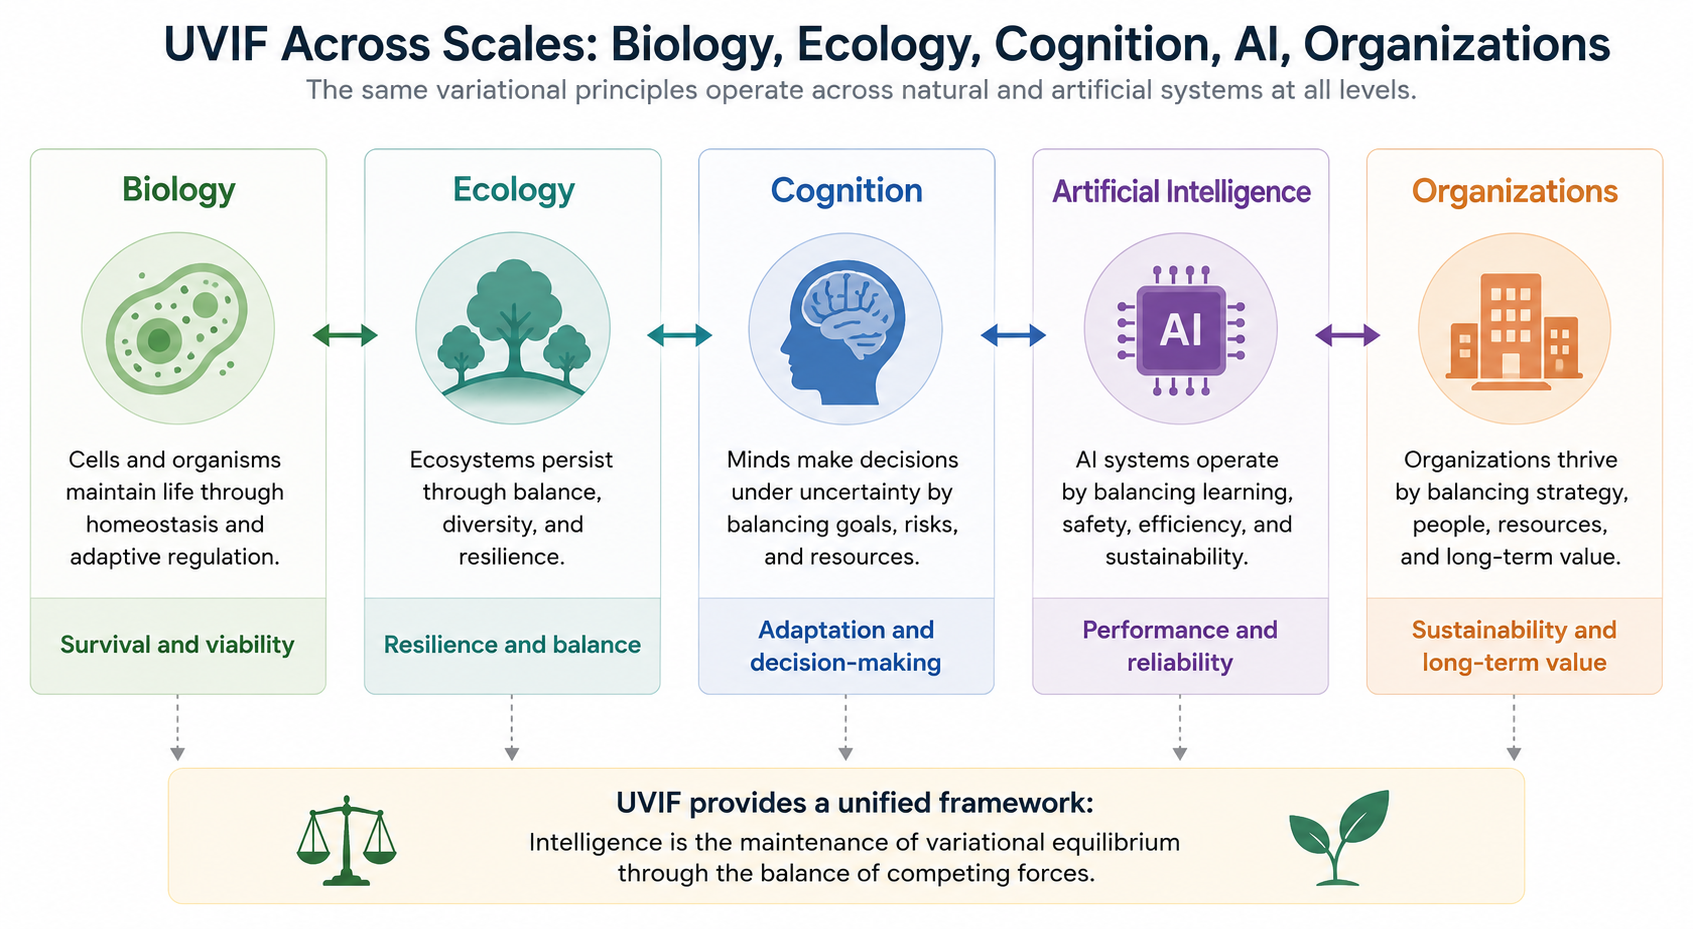
\includegraphics[width=\linewidth]{Figures/Fig5_UVIF_Across_Systems.png}
\caption{UVIF across biological, ecological, cognitive, artificial, and
organizational systems. Although these domains differ in scale and
mechanism, they all maintain functionality through adaptive balance
rather than isolated maximization. UVIF interprets these systems through
a unified variational perspective in which intelligence corresponds to
the maintenance of viable equilibrium under competing pressures,
resource constraints, uncertainty, and environmental change.}
\label{fig:uvif_across_systems}
\end{figure}

The lower part of the figure summarizes the unifying interpretation
provided by \uvif{}. Rather than treating intelligence as isolated
optimization, the framework interprets intelligent operation as the
maintenance of Variational Equilibrium across competing forces. The same
general principle therefore appears across multiple natural and
artificial domains despite their very different physical
implementations.

\subsection{Biological Systems and Physiological Regulation}

The most immediate and compelling validation of the \uvif{} framework
comes from physiology, where the language of force balance and dynamic
equilibrium has described biological function for over a century.

Consider the regulation of blood glucose concentration. The pancreatic
system operates through the opposition of insulin (which drives glucose
into cells, reducing blood concentration) and glucagon (which mobilizes
stored glucose, raising concentration). Neither hormone is simply
maximizing a reward signal; they are opposing forces that jointly
maintain the system within a viable range. When this balance is
disrupted---as in diabetes mellitus---the system fails catastrophically.

In the \uvif{} language, the pancreatic regulatory system instantiates
a Variational Equilibrium: insulin and glucagon correspond to opposing
forces in the force field, and normoglycemia is the equilibrium at
which these forces balance. The admissibility constraints are the
physiological limits beyond which neural and vascular damage occurs.
Adaptive homeostasis corresponds to the shift of the equilibrium
manifold in response to chronic stressors such as chronic
hyperglycemia in diabetes \citep{davies2016adaptive}.

This example generalizes across virtually all physiological regulatory
systems. Thermoregulation balances heat production and dissipation.
Blood pressure regulation balances cardiac output and vascular
resistance. Immune function balances inflammatory and anti-inflammatory
signals. In each case, the system's health is its proximity to
Variational Equilibrium, and disease is the disruption of this
equilibrium \citep{billman2020homeostasis,bich2025homeostasis}.

The evolutionary interpretation is also immediate: organisms that
maintained their Variational Equilibrium across a wide range of
perturbations survived and reproduced; those that were easily
displaced from equilibrium did not. Evolution, in this view, is the
process by which the force field of biological systems has been
refined over billions of years to make Variational Equilibrium
robust \citep{farnsworth2025setpoint,eskov2017homeostasis}.

\subsection{Ecological Systems and Environmental Balance}

Ecosystem dynamics provide the second great testing ground for
\uvif{}. Ecological systems are quintessentially multi-force systems:
predator-prey dynamics, nutrient cycling, competitive exclusion,
mutualism, and succession all involve the opposition and cooperation
of multiple forces acting simultaneously on multiple components
\citep{levin1998ecosystems}.

The canonical predator-prey cycle---where predator and prey
populations oscillate around an equilibrium---is perhaps the simplest
ecological instance of Variational Equilibrium. The predator force
(driving prey population down) and the prey force (driving predator
population down through food limitation) balance at the equilibrium
population densities. The system cycles around this equilibrium rather
than converging to it precisely because biological populations have
finite growth rates and response times---a manifestation of the
homeodynamic principle that equilibria in living systems are dynamic,
not static \citep{lloyd2001homeodynamics}.

More complex ecological systems exhibit higher-dimensional Variational
Equilibria. The spatial self-organization of dryland vegetation
represents a Variational Equilibrium between water competition (a
force driving spatial separation of plants) and facilitation (a force
drawing plants together to share moisture from bare soil)
\citep{kefi2024selforg}. The resulting spatial patterns---bands,
spots, gaps---are the visible signature of this equilibrium, and their
persistence despite ongoing perturbation is evidence of the
equilibrium's stability.

Ecological resilience, in the \uvif{} interpretation, is the size and
robustness of the basin of attraction around the Variational
Equilibrium manifold \citep{gao2016universal,folke2006resilience}.
Systems with high resilience have large basins: they can absorb
significant perturbations and still return to functional equilibrium.
Systems with low resilience are near the edge of their basin: small
perturbations can tip them into a different, possibly dysfunctional,
equilibrium.

The planetary-scale homeostasis hypothesis (the Gaia hypothesis)
represents the most ambitious ecological application of the \uvif{}
framework. The emergence of planetary-scale homeostasis from the
feedback loop between life and the abiotic environment---temperature,
atmospheric composition, ocean chemistry---has been demonstrated in
computational models and provides a striking instance of
self-organized Variational Equilibrium at the highest possible scale
\citep{dyke2013environmental}.

\subsection{Human Cognition and Decision-Making}

Human cognition is the instance of the framework that bears most directly on
the questions of this journal, and it is treated separately and at length in
Section~\ref{sec:cognitive_systems}. In outline, the brain continuously
balances exploration against exploitation, stability against plasticity,
accuracy against metabolic cost, and individual goals against social
constraints; these trade-offs are the cognitive expression of the five
\uvif{} forces, and the manifold along which they are jointly satisfied is the
Variational Equilibrium of cognition.

\subsection{Artificial Intelligence and Adaptive Autonomous Systems}

In artificial intelligence, \uvif{} provides a framework for designing
systems that remain safe, effective, and sustainable across extended
deployment lifetimes. The key insight is that the five forces must all
be explicitly represented in the system's architecture, not collapsed
into a single objective.

A \uvif-aligned AI system for, say, autonomous navigation would not
simply maximize a reward signal for reaching a destination. It would
maintain a force balance between: the epistemic pull to explore
unknown terrain and build better maps; the selective protection of
safety-critical representations (obstacle models, map consistency);
the computational drag that limits onboard processing to available
energy; the action efficiency that selects routes that are both fast
and informative; and the sustainability field that prevents the system
from operating in ways that damage its hardware or deplete its energy
reserves.

The resulting system would not be optimal in the narrow sense of
maximizing any single metric. But it would be robust: capable of
functioning across a wide range of conditions, gracefully degrading
when resources are scarce, and remaining safe even when its models
are uncertain. This is the kind of robustness that the current
paradigm of reward maximization cannot naturally deliver
\citep{garcia2015saferl,yuan2019novel}.

Nature-inspired computing has already drawn on many of these
principles in the design of adaptive algorithms
\citep{jiao2024natureinspired,diaz2025biomimetics}. \uvif{} provides
the unifying theoretical framework that makes these principles coherent
and mutually reinforcing.

\subsection{Societal and Organizational Systems}

The scope of \uvif{} extends naturally to the most complex adaptive
systems that humanity manages: social organizations, institutions,
and economies. These systems face the same fundamental challenge as
biological and ecological systems: how to maintain coherent,
functional operation across time despite continuous internal flux and
external perturbation.

Organizational resilience---the capacity of an institution to absorb
disruption and reorganize while preserving its essential functions---
is the organizational analog of ecological resilience
\citep{ungar2018resilience,folke2006resilience}. Organizations that
achieve long-term resilience do so not by optimizing a single metric
(profit, growth, market share) but by maintaining a force balance
between competing imperatives: efficiency and slack, standardization
and adaptability, short-term performance and long-term investment.

The Integrative Sustainable Intelligence model developed in the
organizational management literature makes a similar argument:
sustainability-oriented organizations must integrate multiple driving
forces rather than subordinating all to a single objective
\citep{silvestre2020integrative,kulkov2023ai}.
Decision-making in organizations that deploy AI must navigate the
competing forces of capability, safety, transparency, and human
oversight \citep{shrestha2019decision}---a challenge that \uvif{}
frames as a problem of maintaining Variational Equilibrium in a
complex socio-technical system.



% Deep revision placeholder inserted.
% [Further conceptual integration recommended]
